\subsection{Estimote}
\label{sec:indoor-positioning:estimote}
We choose to use the solution provided by Estimote for this project.
The choice of Estimote was made due to it being available already, 
having a low price which may fit consumers, 
and its advertised ease of use. 
However, as described further below, the ease of use come at a cost of the accuracy.
Furthermore Estimote has put effort into optimizing their software for indoor positioning, 
and has released a software development kit (SDK),
that developers can use to perform indoor positioning, 
making it easier to adopt the technology.

\subsubsection{The Beacons and the iBeacon Protocol}
Before we describe how we can use the beacons for indoor positioning, 
we want to describe the technology that makes this possible. 
This section is based on a blog post by Estimote on how beacons work \cite{ESTIMOTEBEACON}.

The beacon contains a small ARM processor with an antenna, 
a Bluetooth Smart module and a battery, enclosed in a silicone casing.
A illustration of a beacon is shown by \Cref{fig:estimotebeacon}.
The flat side of the casing has an adhesive on one side, 
so that the beacons can be attached to surfaces. 

\begin{figure}[!htb]
  \centering
  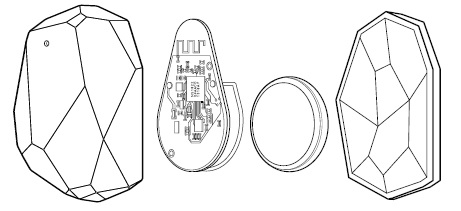
\includegraphics[width=0.6\textwidth]{images/estimotebeacon}
  \caption{Image of an Estimote beacon. Contains a small ARM processor, a Bluetooth Smart module and a battery, enclosed in silicone casing. Source: \protect\cite{ESTIMOTEBEACON}.}
  \label{fig:estimotebeacon}
\end{figure}

The beacons broadcast signals in intervals. 
The beacons can broadcast these in an interval between \SI{100}{\milli\second} and \SI{2000}{\milli\second},
however an operating system such as iOS only scans for signals every \SI{1}{\second}, 
and Android scans every \SI{1.1}{\second}, 
but may changed for faster or slower scans.
Likewise, the beacons can broadcast the signals with a broadcasting power between \num{4} dBm and \num{-30} dBm.
The further the signals travels, the weaker they get.
This means that the further away from a beacon you receive the signal, 
the weaker it is, and thus the accuracy falls. 
In short, the distance estimates will be more accurate the closer to a beacon you are. 

Estimote Beacons uses the iBeacon protocol. 
Each iBeacon packet include \cite{IBEACON}:
\begin{description}
  \item[UUID] A \SI{16}{\byte} identifier string 
  \item[Major] A \SI{2}{\byte} string to identify a subset of beacons within a larger group
  \item[Minor] A \SI{2}{\byte} string meant to identify individual beacons
  \item[Tx Power] A power defined as the signal exactly \SI{1}{\meter} from the device. This is used to estimate the distance between the devices. 
\end{description}

Estimote uses the iBeacon packets to estimate the distances. 
However, rather than trying to estimate exact distances, 
Estimote uses \emph{proximity zones}. 
There are four zones:
\begin{enumerate}
  \item Immediate (very close to the beacon)
  \item Near (about \SIrange{1}{3}{\meter} from the beacon)
  \item Far (further away or the signal is fluctuating too much to make a better estimate)
  \item Unknown 
\end{enumerate}

By using \num{3} or more beacons, it is possible to estimate the users location. 
A typical method of estimating the location is trilateration. 
However, Estimote found that this method could not get better accuracy than \SI{5}{\meter}.
To get better results, 
they utilize particle filtering, sensor fusion and noise reduction algorithms.

\subsubsection{Indoor Location with Estimote}
Estimote, aside from offering the typical use case for beacons like entering a specific region, 
has also specialized in indoor location of users using the iBeacon protocol. 
The company has developed and released the Estimote Indoor Location SDK\footnote{https://github.com/Estimote/iOS-Indoor-SDK}.
They have also released a demo application for iOS\footnote{https://itunes.apple.com/us/app/estimote-indoor-location/id963704810}, 
which is meant to ease configuration needed for indoor location. 

A user will install the beacons in a room by placing a minimum of \num{4} beacons on the walls, 
preferably in the middle of each wall in a rectangular room.   
Next the user walks along the perimeter of the room, 
and thereby registering the location of the beacons, 
by collecting signal strengths from the beacons (a feature of the iBeacon protocol), 
and data from the phones accelerometer and/or gyroscope.
After the configuration, the application will have estimated the length of and placement of the walls, 
along with the signal strengths of each beacon.

To analyze the precision, 
to see whether we could actually use these beacons and Estimote's SDK, 
we performed a few tests. 
During our tests we found that the approach for configuring the indoor positioning, 
as described above, 
works terribly or not at all. 

\Cref{fig:estimote-location-configuration} shows an example of the inaccuracy of Estimote's indoor positioning application. 
\Cref{fig:estimote-location-configuration:estimate} shows the room configured, 
using Estimote's application and \Cref{fig:estimote-location-configuration:actual} shows the same room, 
configured in code using exact measurements of the room. 
Notice the shape of the room changes from being almost quadratic to rectangular;
the short walls are almost \SI{3}{\meter} off.
Also notice that \Cref{fig:estimote-location-configuration:actual} only has \num{4} beacons, 
whereas \Cref{fig:estimote-location-configuration:estimate} has \num{6} beacons. 
We had to install \num{2} additional beacons to detect the ``dent'' in the room's upper left corner. 
Without the \num{2} extra beacons, 
the application would not be able to account for the ``dent'',
which \emph{could} have an impact on the location afterwards. 

\begin{figure}[!htb]%
    \centering
    \subbottom[Room configured with Estimote's application]{\label{fig:estimote-location-configuration:estimate}
        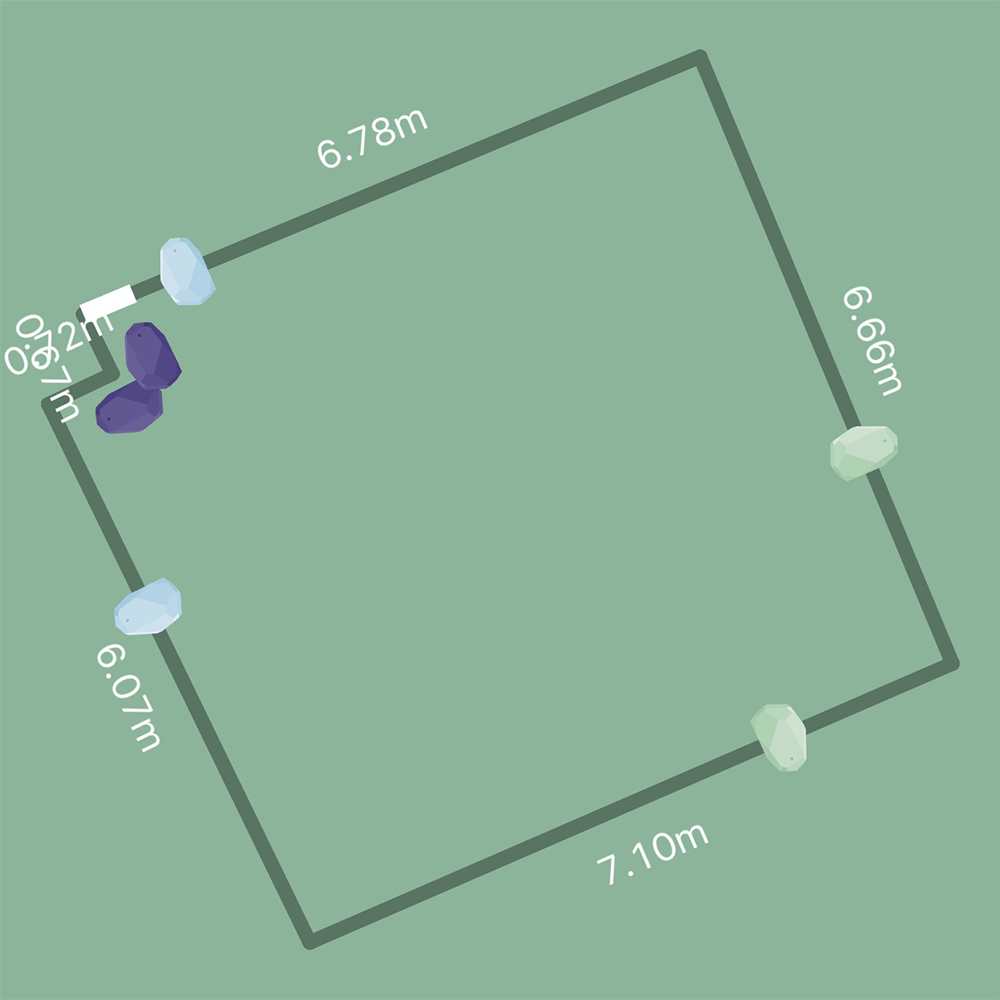
\includegraphics[width=0.45\textwidth]{images/estimote-configurated-room}
    }
    \subbottom[Room configured in code with exact measurements]{\label{fig:estimote-location-configuration:actual}
        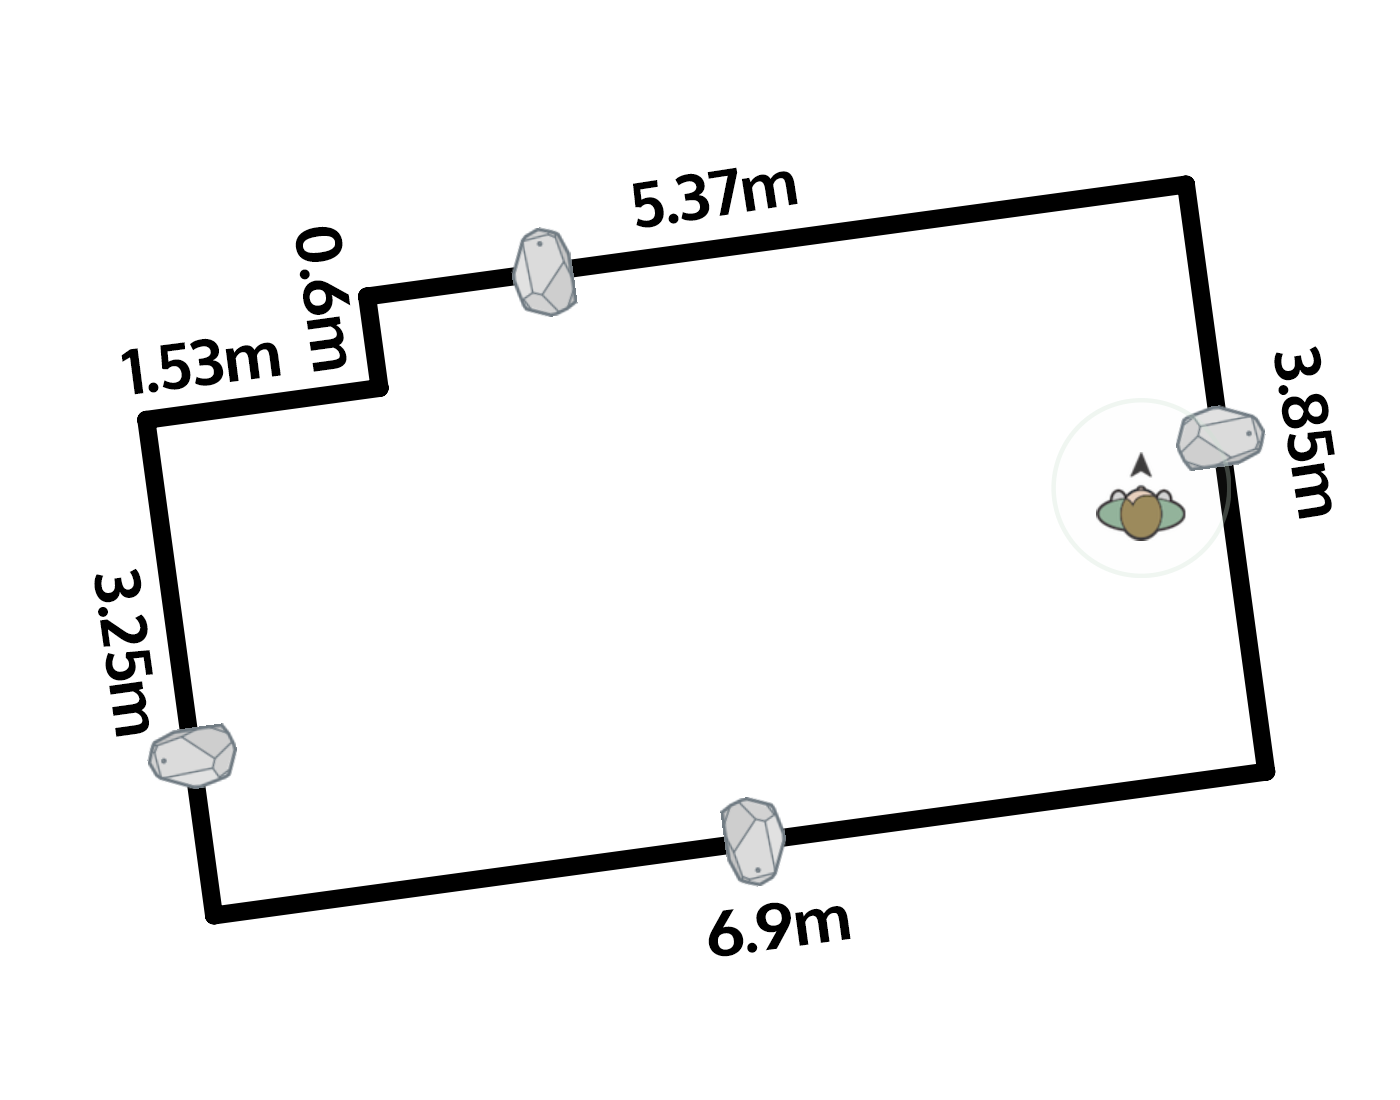
\includegraphics[width=0.45\textwidth]{images/estimote-real-configuration}
    }
    \caption{Illustration of the inaccuracy of the locations configured by Estimote's indoor positioning application.}
    \label{fig:estimote-location-configuration}
\end{figure}

After configuring the room, 
we found the measurements to to be very inaccurate.
Due to this, we decide not to use the built-in room configuration. 

\subsubsection{Configuring Rooms Programmatically}
As mentioned, Estimote provides the Estimote Indoor Location SDK, 
for performing indoor positioning using beacons on iOS. 
The SDK provides two mechanisms for configuring a room for indoor positioning.

\begin{enumerate}
\item Using the built-in controller. The component presents the user with a guided configuration, similar to the one used in the Estimote Indoor Location application.
\item Programmatically using the \texttt{ESTLocationBuilder} class.
\end{enumerate}

The built-in controller was abandoned as it resulted in poor accuracy.

The \texttt{ESTLocationBuilder} lets developers configure a room programmatically, 
by passing coordinates (\texttt{ESTPoint}s) and an orientation to the builder. 
The $X$ and $Y$ value of each coordinate is measured in meters. 
Therefore a set of coordinates $\{(0, 0), (0, 5)\}$ represents a horizontal line of $5$ meters, 
and the set of coordinates $\{(0,0),(0,5),(5,5),(5,0)\}$ represents a $5$ by $5$ meter room.

\Cref{fig:estlocationbuilder-livingroom} shows an example of a location created programmatically using the \texttt{ESTLocationBuilder}. The room is created using the following set of coordinates: $\{(0, 0), (5.37, 0), (5.37, 0.6), (6.9, 0.6), (6.9, 3.85), (0, 3.85)\}$.

\begin{figure}[!htb]
  \centering
  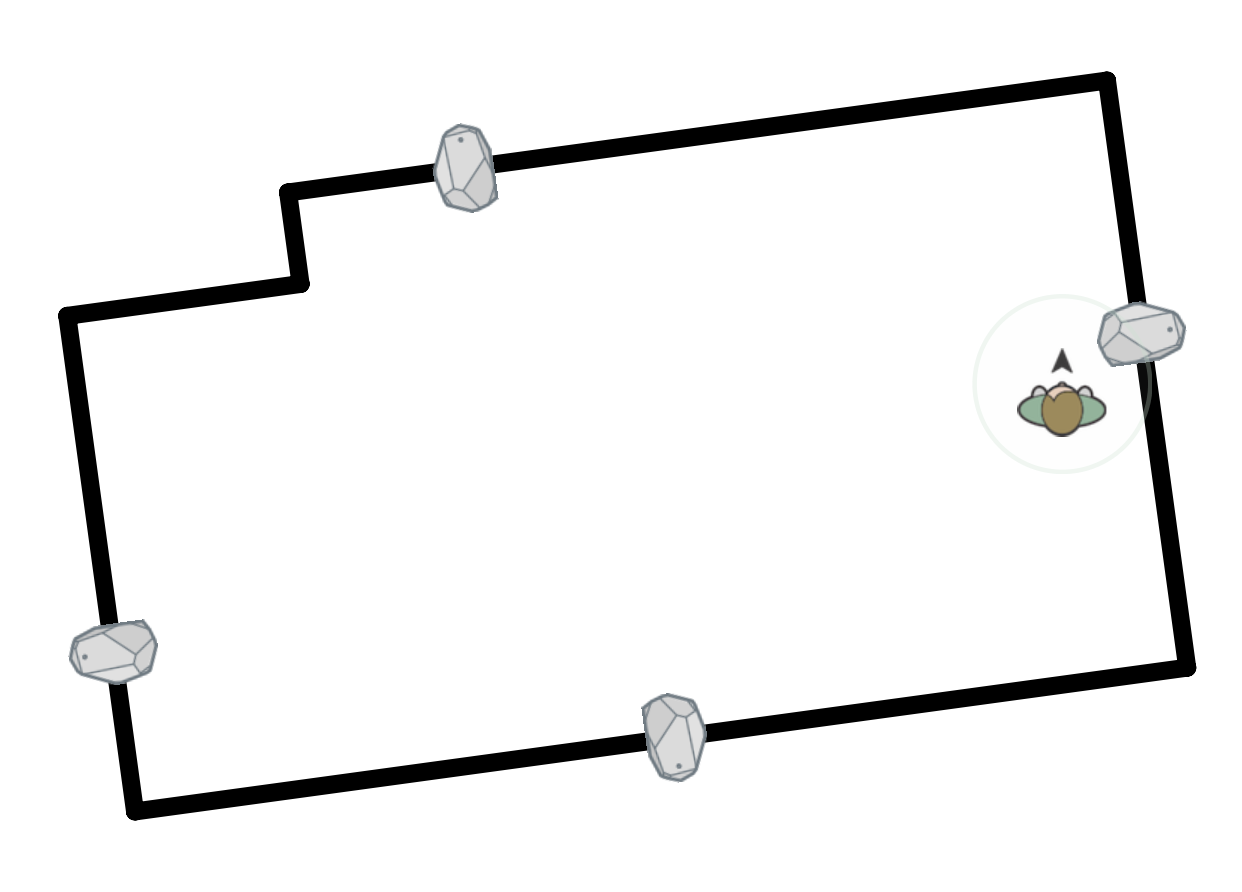
\includegraphics[width=0.33\textwidth]{images/living-room}
  \caption{Location created using the \texttt{ESTLocationBuilder}. Note that the model is rotated accordingly to the orientation of the room and the position of north relative to the user.}
  \label{fig:estlocationbuilder-livingroom}
\end{figure}

The builder is configured with \num{6} coordinates that gives information about the shape of the room. 
Next, the beacons are added to the walls of the room. 
Beacons are added with the MAC address of the beacon.
Lastly the orientation of the room relative to north and the name of the room is set. 
When the room has been configured, 
it can be stored on the users Estimote account using the Estimote SDK.
Using the \texttt{ESTLocationBuilder} to model a room reduces any uncertainties in estimating the users location, 
caused by an imprecise model of the room.

%%% Local Variables:
%%% mode: latex
%%% TeX-master: "../../master"
%%% TeX-command-extra-options: "-shell-escape"
%%% End:
